\section{Validierung}

\subsection{Hardware}

\subsubsection{Messschaltung}
Die Validierung der Messschaltung gestaltet sich durchaus einfach, da die beiden Formeln für die erwarteten Messwerte $messU$ (\ref{eq:messU}) und $messI$ (\ref{eq:messI}) bekannt sind. Problematisch an diesen beiden Formeln ist jedoch, dass mit idealen Bauteilen gerechnet wurde, welche in der Realität nicht verfügbar sind. Bei der Spannungsmessung sind dies lediglich die Toleranzen für die Widerstandswerte, sodass sich bei Widerständen mit 1\% Genauigkeit ein maximaler Fehler von 2.02\% bemerkbar machen kann. Dieser Fehler setzt sich jedoch linear fort, sodass weiterhin durch einen konstanten Faktor dividiert werden kann. Die dazugehörige Messreihe ist im Anhang unter \ref{subsec_messu} auf Seite \pageref{subsec_messu} aufgeführt.

Bei der Strommessung sind es sämtliche Widerstände, die beiden Operationsverstärker sowie der Hallsensor, welche Toleranzen aufweisen. Die beiden 1k$\Omega$ Widerstände, welche die Subtrahendensspannung von Vcc/2 erzeugen, würden dabei einen Offset erzeugen, welcher in der nachfolgenden invertierenden Verstärkerschaltung noch verstärkt wird. Die Toleranzen der anderen Widerstände sowie die Toleranz des Hallsensors wirken dabei als ein konstanter Vorfaktor. Der Offset sowie der Vorfaktor wurden im Anhang unter \ref{subsec_messi} auf Seite \pageref{subsec_messi} mittels einer Messreihe bestimmt.

In den Tests funktionierten die einzelnen Schaltungsteile. Das Zusammenspiel mit der restlichen Schaltung verursacht jedoch vor allem bei der Strommessung noch grössere Probleme, sodass dort weitere Zeit zur Fehlersuche investiert werden müsste.

\subsubsection{Regler}\label{subsec:ValRegler}

Zur Validierung des Reglers wurde der Ausgangsstrom sowie die Ausgangsspannung bei maximaler Aussteuerung und variablem Ausgangs-Widerstand gemessen. Dabei kommt die Stromlimitierung nicht vom Schaltregler selbst, sondern von der zu testzwecken verwendeten Quelle. Ausserdem wurden Strom und Spannung im Verhältnis bei drei verschiedenen Lastwiderständen gemessen, siehe Abbildung \ref{fig::Reglermessung}. Die genauen Messreihen finden sich im Anhang unter \ref{ValidMeas}\colorbox{red}{BITTE ANHANG ERGÄNZEN} auf Seite \pageref{ValidMeas}.

\begin{figure}[h]
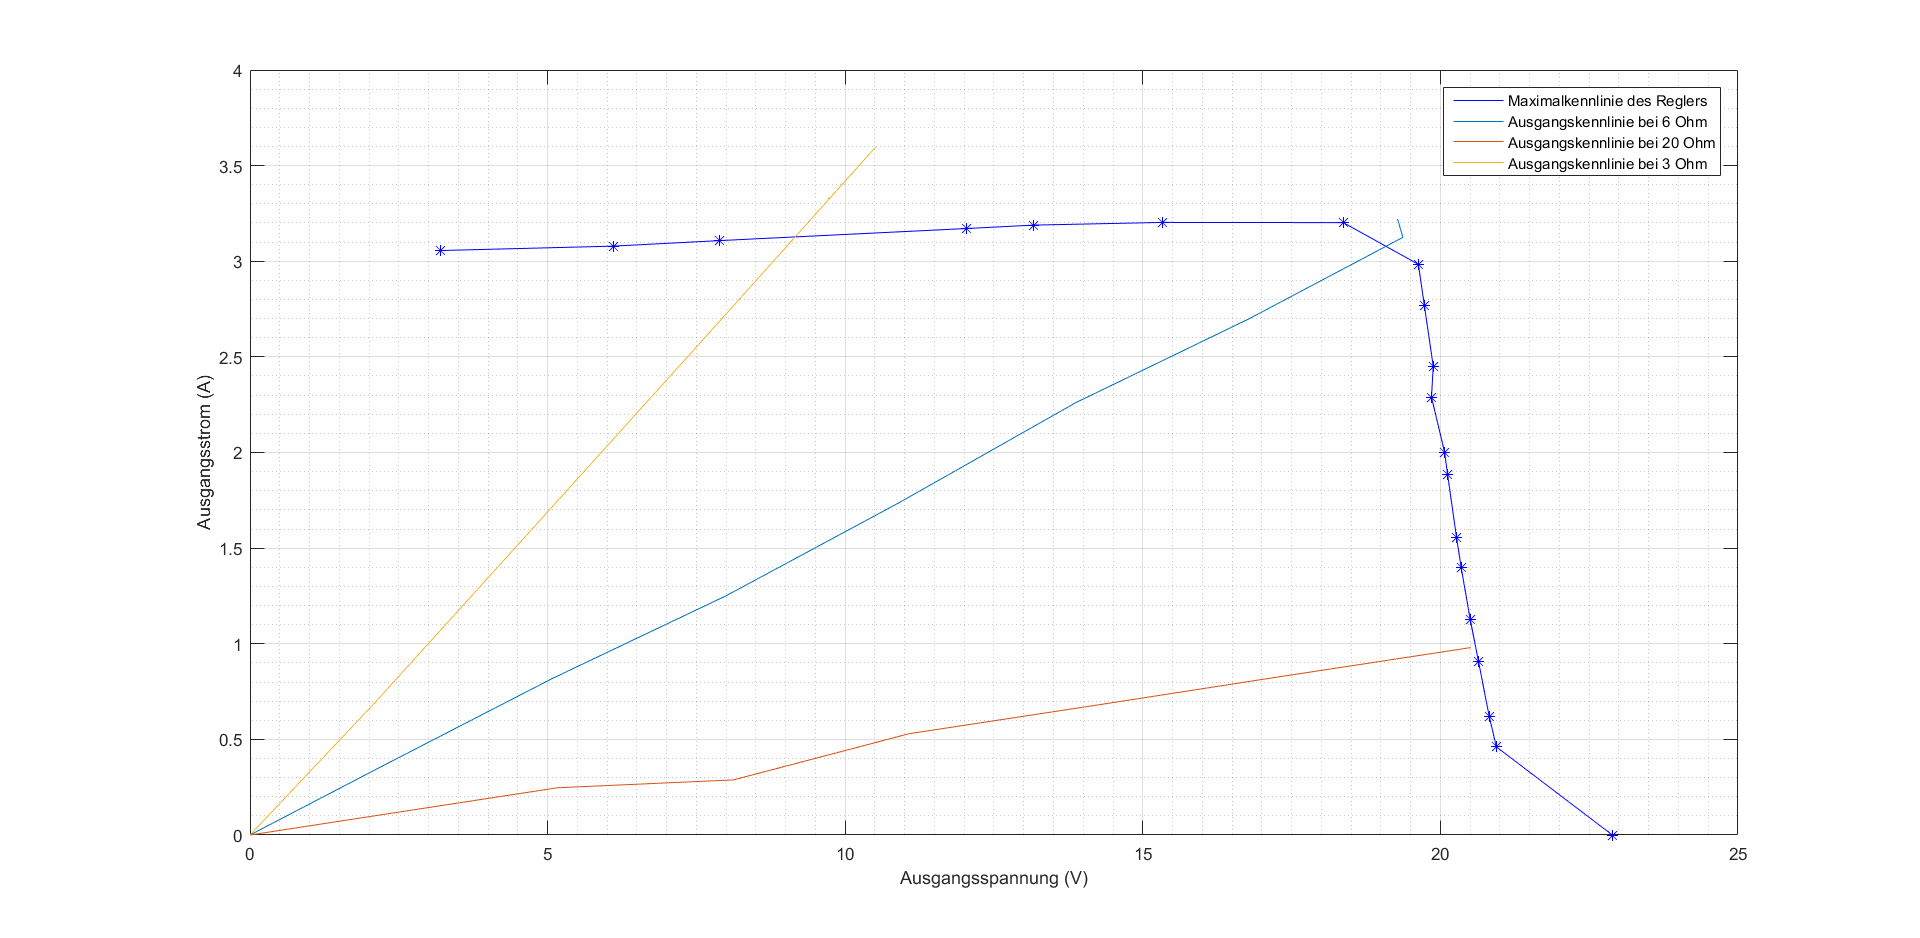
\includegraphics[width=1.0\textwidth]{ReglerMessung.png}%
\caption{Messung der Ausgangskennlinien graphisch dargestellt.}
\label{fig::Reglermessung}
\end{figure}

Der Kurzschlussstrom konnte nicht gemessen werden, da der Regler sich zu stark erwärmte und unbrauchbar wurde.

Auch wurde die Effizienz des Reglers sowie der Rippel gemessen.
Bei der Messung der Rippelspannung wurde festgestellt, dass diese im Bereich 2.5-1.3V Feedbackspannung mehr als 5\% beträgt.
%Dieser Bereich entspricht beinahe dem Kurzschlussfall, bei welchem auch weitere Probleme auftreten \todo{Richtig so? Das von dir war falsch ;)}. 
Um dies zu korrigieren gibt es mehrere Möglichkeiten: Man kann einen grösseren Ausgangskondensator verwenden oder die Spulengrösse verändern. Es ist zudem noch anzumerken, das in dieser Messschaltung kein zusätzliches Ausgangsfilter verwendet wurde (zu sehen in Grafik \ref{fig::LTSchemata}), welches den Rippel der Ausgangsspannung auch verbessern würde. In diesem Bereich ist auch der Wirkungsgrad klein. Er beträgt ca. 50\% in diesem Bestrahlungsbereich, in den anderen Bereichen ca. 70-80\% (siehe Messreihe im Anhang \ref{ValidMeas}.

\paragraph{Bei der Hardware müssten für eine korrekte Funktion folgende Verbesserungen vorgenommen werden:}
\begin{itemize}
	\item Am Ausgang des Operationsverstärkers für die Strommessung (siehe Abbildung \ref{fig:Messschaltung_I}, dort als $messI$ bezeichnet) ist die Spannung zum Teil in einem undefinierten Zustand. Es wird vermutet, dass diese Störung von der ebenfalls auf dieser Platine erzeugten 5V-Hilfsspannung kommen. Bei Tests mit externer Spannungsspeisung konnten diese Fehler nicht nachvollzogen werden.
\end{itemize}